\section{Zielsetzung}
Ziel des Versuches ist die Untersuchung der Temperaturabhängigkeit der thermischen Elektronenemission und die 
Bestimmung der materialspezifischen Austrittsarbeit von Wolfram. 

\section{Theorie}
\label{sec:Theorie}


\subsection{Austrittsarbeit}
In der Gitterstruktur eines Metalls sind die Elektronen nicht an einzelne Atome gebunden. Daher können die Potentiale inner- und außerhalb als konstant angenommen werden. 
Das innen liegende Potential ist geringer als das äußere. \\
Um das Metall zu verlassen muss also eine bestimmte Energie aufgewendet werden. \\
Diese wird als Austrittsarbeit bezeichnet und durch $W_A = e_0 \phi$ berechnet.
Hier ist $\phi = \Phi_A - \Phi_I$ die Differenz zwischen innerem und äußeren Potential und $e_0$ die Elementarladung. 

  

\subsection{Richardson-Gleichung}
Die Sättigungsstromdichte beschreibt die Anzahl der Elektronen, die das Metall je Zeit- und Flächeneinheit verlassen. \\
Die Abhängigkeit der Sättigungsstromdichte $j_{\symup{S}}(T)$ von der Temperatur wird durch die Richardsongleichung
\begin{equation}
  j_{\symup{S}}(T) = 4 \pi \frac{e_0 m_0 k^2}{h^3} T^2 \exp\left(\frac{-e_0 \phi}{k T} \right),
  \label{eq:richardson}
\end{equation}
mit der aus der Temperatur $T$ sowie den Konstanten $e_0$ (Elementarladung),
$m_0$ (Elektronenruhemasse), $k$ (Boltzmann-Konstante) und
$h$ (Planksches Wirkungsquantum) beschrieben.\\

\subsection{Langmuir-Schottkysche Raumladungsgleichung}
Der Anodenstrom der Diode ist abhängig von der Anodenspannung.\\
Bei zu geringer Anodenspannung werden nicht alle Elektronen ausreichend beschleunigt, um die Anode zu erreichen. 
Daher ist der Anodenstrom ab einem Schwellwert unabhängig von der angelegten Spannung.\\
Damit ist das Ohmsche Gesetz für Dioden ungültig. \\
Stattdessen wird eine neue Gesetzmäßigkeit aus der Kontinuitätsbedingung 
\begin{equation*}
j = - \rho v
\end{equation*}
hergeleitet. Hier ist $j$ die Stromdichte, $v$ die Strömungsgeschwindigkeit und $\rho$ die Ladungsdichte.\\
Zusammen mit der Poissongleichung
\begin{equation*}
\Delta V = - \frac{1}{\epsilon_0} \rho
\label{eq:poisson}
\end{equation*}
mit Potential $V$ und elektrischer Konstante $\varepsilon_0$ und der Energieerhaltung $E_{pot}=E_{kin}$ wird das Potential 
\begin{equation*}
  U(x) = \left(\sqrt{\frac{j}{4\epsilon_0\sqrt{\frac{2e}{m}}}}x\right)^{\frac{4}{3}}.
  \end{equation*}
bestimmt. Hier ist x die Ortskoordinate.\\ 
Es folgt für die Stromdichte das Langmuir-Schottkysche Raumladungsgesetz 
\begin{equation}
  j (\Phi_A)= \frac{4}{9} \symup{\epsilon_0} \sqrt{\frac{2\symup{e_{0}}}{m_{0}}} \frac{\Phi_A^{\frac{3}{2}}}{a^2} \,.
  \label{eq:lang}
\end{equation}

\subsection{Hochvakuumdiode}
Die Messung wird mit der Hochvakuumdiode durchgeführt. Das Vakuum ist notwendig, da die Elektronen sonst mit den Luftmolekülen
wechselwirken würden. \\
Im Gerät wird ein Draht, in diesem Fall aus Wolfram, durch einen Strom erhitzt. Die dort emittierten Elektronen werden durch
die angelegte Saugspannung in Richtung der Anode beschleunigt, an der der Anodenstrom gemessen wird. Ein schematischer Aufbau der beschriebenen Apparatur ist in \autoref{fig:hochvdiode} zu sehen.

\begin{figure}[H]
  \centering
  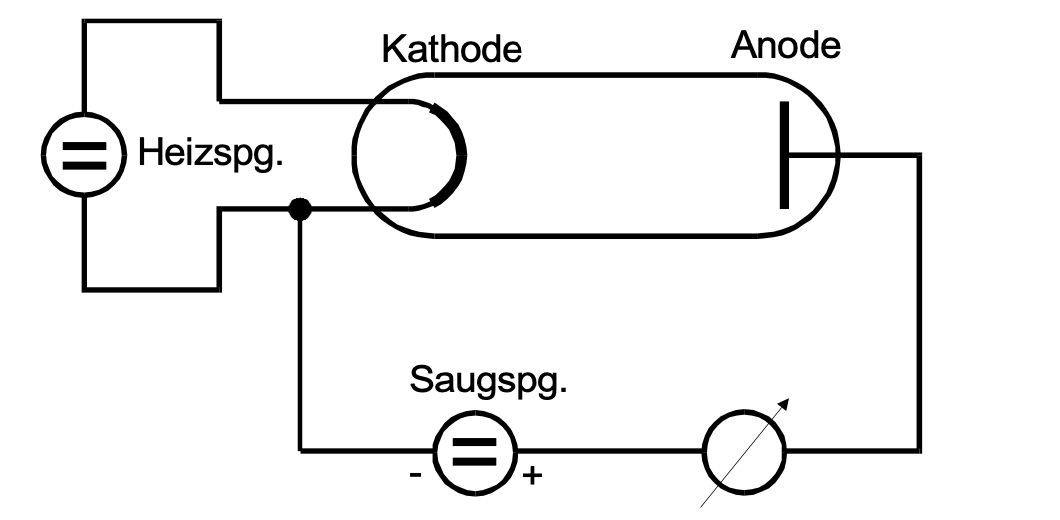
\includegraphics[width=5cm]{content/hochvdiode}
  \caption{Schematische Darstellung einer Hochvakuumdiode.\cite{sample}}
  \label{fig:hochvdiode}
\end{figure}
Der Zusammenhang zwischen Anodenstrom und Saugspannung kann wie in \autoref{fig:kenn} graphisch durch die sogenannte Kennlinie dargestellt werden.\\
Die Kennlinie kann in drei Abschnitte unterteilt werden.
Das Anlaufstromgebiet der Kennlinie wird im nächsten Abschnitt genauer untersucht.
\begin{figure}[H]
  \centering
  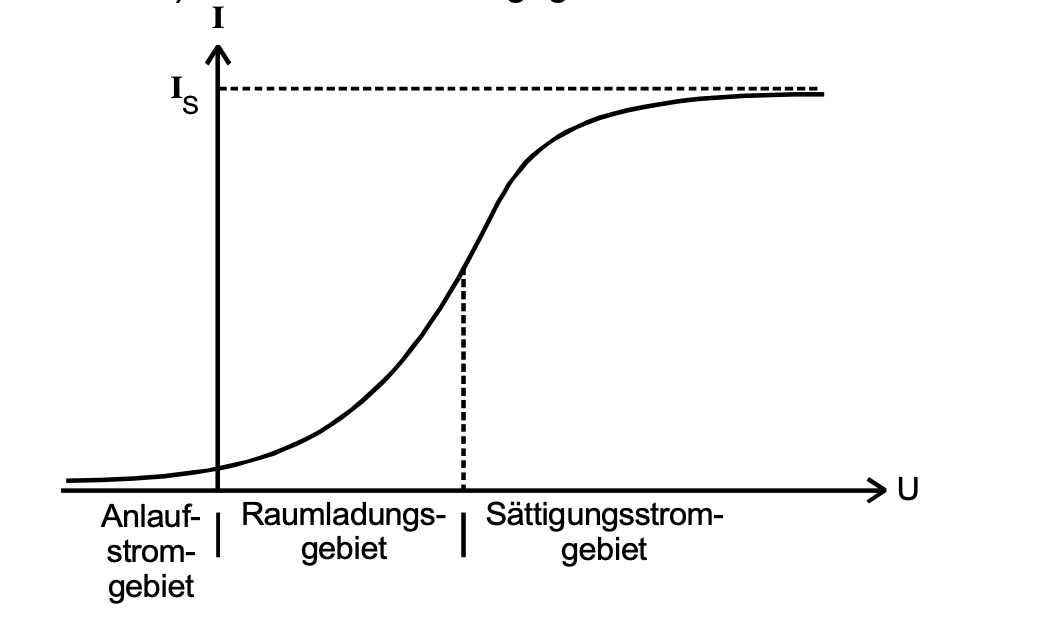
\includegraphics[width=5cm]{content/kenn}
  \caption{Kennlinie einer Hochvakuumdiode.\cite{sample}}
  \label{fig:kenn}
\end{figure}


\subsection{Anlaufstromgebiet}


\begin{figure}
  \centering
  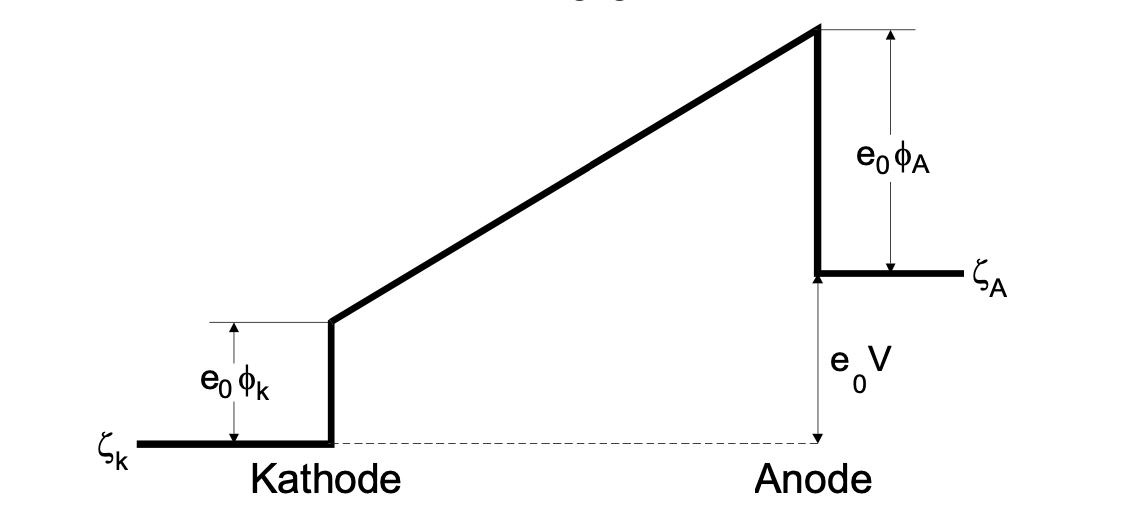
\includegraphics[width=\textwidth]{content/potential}
  \caption{Diagramm der Potentialverhältnisse der Diode im Bereich des Anlaufstromgebietes.\cite{sample}}
  \label{fig:potential}
\end{figure}

Theoretisch sollte nach \autoref{eq:lang} ohne angelegte Spannung auch kein Anodenstrom zu messen sein. \\
Im Experiment zeigt sich jedoch der sogenannte Anlaufstrom. 
Er wird durch Elektronen erzeugt, deren Energie die Austrittsenergie übersteigt. \\
Um die Anode zu erreichen, muss die Energie mindestens $E \geq e_0 (\phi + U)$ betragen.
Mit \autoref{fig:potential} lässt sich die Anlaufstromstärke 
\begin{equation}
  j(\Phi_A)= j_0 \cdot e^{- \frac{e_0(\phi_A + U)}{kT}} \propto e^{- \frac{e_0 U}{kT}}
\end{equation} 
herleiten. 




